\PassOptionsToPackage{unicode, colorlinks=true, linkcolor=black, urlcolor=black}{hyperref}
\documentclass[t, table]{beamer}

%% load the theme with the correct option for your institute
%% currently supported are tudo and ethz
\usetheme{fact}

\usepackage[
  orientation=portrait,
  size=a0,
  scale=1.0,  % scale fonts with this factor
]{beamerposter}

\usepackage{fontspec}
\usepackage{polyglossia}
\setmainlanguage[variant=american]{english}

% microtypographic adjusments (protrusion, kerning etc.)
\usepackage{microtype}

% automatic enquoting depending on the language with \enquote{Bla}
\usepackage{csquotes}

% for the qrcode
\usepackage{qrcode}

% math setup
\usepackage{mathtools}
\usepackage{unicode-math}
\setmathfont[Scale=MatchLowercase]{TeX Gyre Pagella Math}

\usepackage{xfrac}
\usepackage[
  detect-weight=true,
  binary-units=true,
  per-mode=fraction,
  fraction-function=\sfrac
 ]
 {siunitx}
% some stupid sample text to fill the boxes
\usepackage{blindtext}

% offers the \begin{multicols}{NCOLS} environment
\usepackage{multicol}

% for including all types of graphics
\usepackage{graphicx}

\usepackage{tabularx}

% bibliography settings
\usepackage[
  backend=biber,
  style=numeric,
  url=false,
  sorting=none,
  firstinits=true,
]{biblatex}
\DeclareFieldFormat*{title}{\textit{#1}}


\newcommand{\stf}{\texttt{streams-framework} }
% a little complicated, but this creates an inline list.
\renewcommand*{\bibfont}{\footnotesize}
\addbibresource{references.bib}
\defbibenvironment{bibliography}
  {\noindent}
  {\unspace}
  {}
\renewbibmacro*{begentry}{%
  \usebeamercolor{bibliography item}%
  \color{bibliography item.fg}%
  \printtext[labelnumberwidth]{%
    \printfield{prefixnumber}%
    \printfield{labelnumber}%
  }%
  \setunit{\addnbspace}%
}
\renewcommand*{\finentrypunct}{\addperiod\space}

% just a helpful definition to get columns with a third of the textwidth
\newlength{\thirdtextwidth}
\setlength\thirdtextwidth{0.333333\textwidth}


\title{Real Time Streaming Analysis of IACT Data}
\author{Kai Brügge \large{for the FACT-Collaboration}}
\newfontfamily{\firathin}{fira sans thin}
\usetikzlibrary{calc}
\usetikzlibrary{shadows.blur}

\begin{document}%

% nix abstract
% \begin{columns}[onlytextwidth]%
%   \begin{column}{\textwidth}%
%     \begin{block}
%       \blindtext[2]
%     \end{block}
%   \end{column}%
% \end{columns}%

\begin{multicols}{2}
    \begin{block}[equal height group=B]{CTA - The Cherenkov Telescope Array}%
      \begin{multicols}{2}
        \begin{figure}
          \includegraphics[width=\linewidth]{images/cta.png}\\
          % \caption{The FACT Telescope during a calibration procedure \cite{fact-performance}}
        \end{figure}
        \columnbreak
        Once completed, the  Cherenkov Telescope Array (CTA)  will be able to map the gamma-ray sky
        in a wide energy range from several tens of GeV to some hundreds of TeV and will be more sensitive
        than previous experiments by an order of magnitude.

        CTA will consist of approximately 100 telescopes of different sizes and designs.
        Telescope data will be streamed via network from the telescopes to a central computing facility
        on-site.
      \end{multicols}
    \end{block}%

    \begin{block}[equal height group=B]{Real Time Requirements of CTA}%
      \begin{multicols}{2}
        \begin{figure}
          \includegraphics[width=\linewidth]{images/cta.png}\\
          % \caption{The FACT Telescope during a calibration procedure \cite{fact-performance}}
        \end{figure}
        \columnbreak
          The \texttt{streams-framework} is a data streaming environment written in Java.
          The purpose of the streams-framework is to provide an abstract way to model the data flow of an application.
          It comes with a number of fundamental building blocks to define a data flow graph using an Extensible Markup Language (XML) based description.
          The FACT-Tools are a collection of tools build on top of the \texttt{streams-framework} which reduce FACT raw data into image parameters that
          can be used for supervised machine learning methods.
      \end{multicols}
    \end{block}%


    \begin{block}[equal height group=A]{Multivariate Signal/Background Seperation}%
      \begin{multicols}{2}
        \begin{figure}
          \includegraphics[width=\linewidth]{figures/angular_resolution.pdf}\\
          % \caption{Toller Plot.\cite{fact-performance}}
        \end{figure}
        \columnbreak
        Supervised machine learning is used to seperate signal events from background.
        Simulated, labeled, data is used to train the models.
        A RandomForest classifier with \num{150} trees is
        used as a model for the Real Time Analysis presented here. A total of \num{52} features are used
        while training the model. All are calculated using the FACT-Tools.
        The popular Python machine learning library scikit-learn is used to train and then
        store the models into the PMML format. This way the stored model can be shared
        between programming languages and applied to the data stream from the telescope.

        % Data handling is performed by the Pandas library [28], using data frames inspired by the R programming language.
        % Visualizations are created by the Matplotlib [22] Python library.


      \end{multicols}
    \end{block}%

    \begin{block}[equal height group=A]{Multivariate Energy Estimation}%
      \begin{multicols}{2}
        \begin{figure}
          \includegraphics[width=\linewidth]{figures/impact_estimator.pdf}\\
          % \caption{Toller Plot.\cite{fact-performance}}
        \end{figure}
        \columnbreak
        Online energy estimation for the Real Time Analysis works in a similar fashion to the online separation.
        A Random Forest regressor with \num{150} trees is used to estimate the event energy.
        The regressor is trained on the same set of variables as the separator.
        Using no additional cuts the leads to an energy resolution which is on par with more complicated
        offline methods. Both the bias and the resolution of the estimator are strongly dependent on the simulated energy.
        Low energy showers create smaller images in the camera since they do not emit as much Cherenkov radiation as their high energy counterparts.
      \end{multicols}
    \end{block}%

    % \begin{alertblock}[equal height group=A]{Test}%
    %   \begin{multicols}{2}
    %     \blindtext\cite{fact-reference}
    %     \blindtext
    %   \end{multicols}
    % \end{alertblock}%





    % \begin{alertblock}[equal height group=A]{Test}%
    %   \begin{multicols}{2}
    %     \blindtext\cite{fact-reference}
    %     \blindtext
    %   \end{multicols}
    % \end{alertblock}%




    \begin{block}[equal height group=A]{Monitoring Gamma-Ray Sources}%
      \begin{multicols}{2}
        \begin{figure}
          \includegraphics[width=\linewidth]{figures/angular_resolution_vs_energy.pdf}\\
          % \caption{Toller Plot.\cite{fact-performance}}
        \end{figure}
        \columnbreak
        One of FACT’s main goals is the long-term monitoring of bright AGN type gamma ray sources.
        These sources can show variable behavior in terms of both total brightness and spectral properties.
        IACTs record so-called light curves which show the gamma ray  flux versus time.
        In case a source shows a sudden increase in  flux, it is considered to be in a flaring state.
        In case a  flare is detected, FACT can alert other experiments to trigger multi-wavelengths observations.
        The figure to the left shows excess rates of the AGN Markarian 421 over time.
        A flare on the 25th of June is clearly visible.
      \end{multicols}
    \end{block}%

% ------------------Next columns -----------------
% ------------------------------------------------
    \columnbreak

        \begin{center}

        \begin{streamblock}[equal height group=C, width=0.6\linewidth]{0mm}{-5mm}{}%
          \begin{multicols}{2}
            \begin{figure}
              \includegraphics[width=\linewidth]{images/cta.png}
            \end{figure}
            \columnbreak
            The telescope emits \num{50} events per second on average. This leads to a mean data rate of \SI{43.2}{\mega \byte} per second and up to
            \SI{1}{\tera \byte} of collected raw data per night.
          \end{multicols}
        \end{streamblock}%

        \begin{streamblock}[equal height group=C, width=0.6\linewidth]{-5mm}{-5mm}{}%
          \begin{multicols}{2}
            \begin{figure}
              \includegraphics[width=\linewidth]{figures/theta.pdf}
            \end{figure}
            \columnbreak
            Calibration data is applied to the data stream to convert raw sensor output to physical units. This is the most time consuming step and
            is paralellized to several CPUs.
          \end{multicols}
        \end{streamblock}%

        \begin{streamblock}[equal height group=C, width=0.6\linewidth]{-5mm}{-5mm}{}%
          \begin{multicols}{2}
            \begin{figure}
              \includegraphics[width=\linewidth]{figures/crab_efficiency.pdf}
            \end{figure}
            \columnbreak
              The number of photons and their respective arrival times are extracted from the raw data. Camera pixels not containing
              any cherenkov photons are dropped.
          \end{multicols}
        \end{streamblock}%

        \begin{streamblock}[equal height group=C, width=0.6\linewidth]{-5mm}{-5mm}{}%
          \begin{multicols}{2}
            \begin{footnotesize}
            \begin{figure}
              \begin{tikzpicture}[
                  sibling distance= 5em,
                  level distance  = 3em,
                  % edge from parent/.style = {draw,},
                  text centered,
                  every node/.style = {shape=rectangle, sharp corners, draw, align=center, minimum size=1cm, text width=2cm}
                ]
              \node {Width}
                child { node {Length} }
                child { node {Size}
                  child { node {Arrival}
                      child { node {Delta} }
                      child { node {Alpha} }
                    }
                  };
              \end{tikzpicture}
            \end{figure}
          \end{footnotesize}
            \columnbreak
            Multivariate models trained on simulated data are applied to the data stream online. Energy estimation and
            background suppression is performed to label the data coming from the telescope.
          \end{multicols}
        \end{streamblock}%


        \begin{streamblock}[equal height group=C, width=0.6\linewidth]{-5mm}{0mm}{}%
          \begin{multicols}{2}
            \rowcolors{2}{gray!25}{white}
            {\color{maincolor}
            \begin{tabularx}{\linewidth}{cXc}
              \rowcolor{gray!50}
                \textbf{Length} & \textbf{Energy} & \textbf{Label} \\
                30 & 2   TeV & $g$   \\
                15 & 200 GeV & $p$  \\
                29 & 450 GeV & $p$  \\
                40 & 900 GeV & $g$ \\
                35 & 10 GeV & $g$ \\
                10 & 13 GeV & $p$
            \end{tabularx}
            }

            \columnbreak

            Results of the analysis are stored on-site in \texttt{fits} files and into an SQL Database.
            A webserver provides public access to high-level results in real time.
          \end{multicols}
        \end{streamblock}%

        \vspace{5cm}
        \tikz[]{
          \node[anchor=north]{\includegraphics[width=0.6\linewidth]{images/cta.png}};
          % \node[scope fading=south, anchor=north]{\includegraphics[width=0.6\linewidth]{images/website.png}};

        }

      \end{center}





% \begin{tikzpicture}[overlay, shift={(60 cm, 75 cm)}, anchor=north west]
%       \definecolor{sourceGreen}{HTML}{77cc5a}
%       \definecolor{sinkRed}{HTML}{c45858}
%
%       \pgfmathsetmacro{\scale}{2};
%       \pgfmathsetmacro{\sourceWidth}{5*\scale};
%       \pgfmathsetmacro{\sourceHeight}{5*\scale};
%       \pgfmathsetmacro{\cubeSize}{3*\scale};
%       \pgfmathsetmacro{\circleSize}{1*\scale};
%       \pgfmathsetmacro{\textShift}{2.5*\scale};
%
%       \tikzset{every node/.style={rectangle, draw=black!80,fill=gray, text=white, rounded corners=0.5pt, ultra thin, font=\fontsize{36}{36}\firathin,},
%                     processorshape/.style={minimum width=\sourceHeight cm,minimum height=\cubeSize cm},
%                     queueshape/.style={minimum width=\cubeSize cm,minimum height=\cubeSize cm },
%                     sink_anchor/.style = {circle, draw=sinkRed, fill=sinkRed, minimum size=\circleSize cm, line width = 0.1cm,
%                                                             blur shadow={shadow xshift=-0.07cm, shadow yshift=-0.07cm}
%                                                         },
%                     }
%
%
%       \node[processorshape] (processor_1) at (0, 0) {Processor};
%
%       \node[processorshape] (processor_2) at (0, -10) {Processor};
%
%       \node[processorshape] (processor_3) at (0, -20) {Processor};
%
%
%       % \draw node[vertex] (Joint) at (1,0) {};
%
%       \draw[-,draw=gray] (processor_1) to (processor_2);
%       \draw[-,draw=gray] (processor_2) to (processor_3);
%
%       % \node[source_anchor](anchor_1) at (1.8,-1){};
%     \end{tikzpicture}



\end{multicols}


\vfill
\begin{columns}[t, onlytextwidth]%
  \begin{column}{0.42\textwidth}%
    \begin{block}[equal height group=bottom]{\normalsize References}
      \footnotesize%
      \printbibliography%
    \end{block}
  \end{column}%
  \begin{column}{0.42\textwidth}%
    \begin{block}[equal height group=bottom]{\normalsize Acknowledgment}
      \begin{multicols}{2}%
        \footnotesize
        Part of this work is supported by Deutsche Forschungsgemeinschaft (DFG) within the Collaborative Research Center SFB 876
"Providing Information by Resource-Constrained Analysis", project C3. 

      \end{multicols}%
    \end{block}
  \end{column}%
  \begin{column}{0.16\textwidth}%
    \begin{block}[equal height group=bottom]{\normalsize Contact}
      \begin{columns}%
        \begin{column}{0.33\textwidth}
          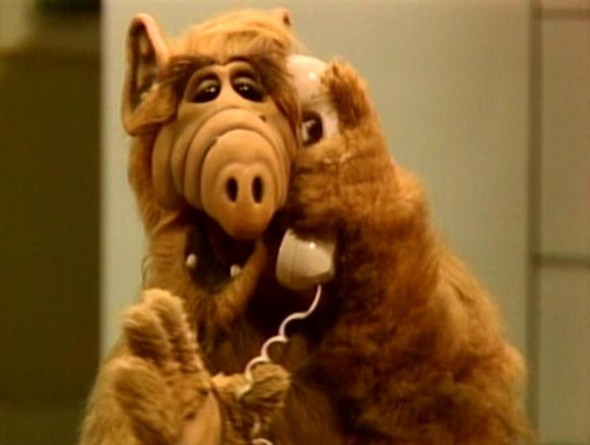
\includegraphics[width=\linewidth]{images/alf.jpg}
        \end{column}
        \begin{column}{0.65\textwidth}
          \footnotesize
              Kai Brügge, \\
              Astroparticle Physics, \\
              TU Dortmund \\
              \texttt{kai.bruegge@udo.edu}
        \end{column}

      \end{columns}
    \end{block}
  \end{column}%
\end{columns}%
\end{document}
